\subsection{Three (and more) Transistor Circuits}

In the following, we will turn to some slightly more complex circuits in order to introduce the principles of the transconductance amplifier, which is used in a variety of circuit configurations in analog circuit design.

\subsubsection{The differential pair}
\label{section:diffpair}
\begin{figure}[H]
    \centering
    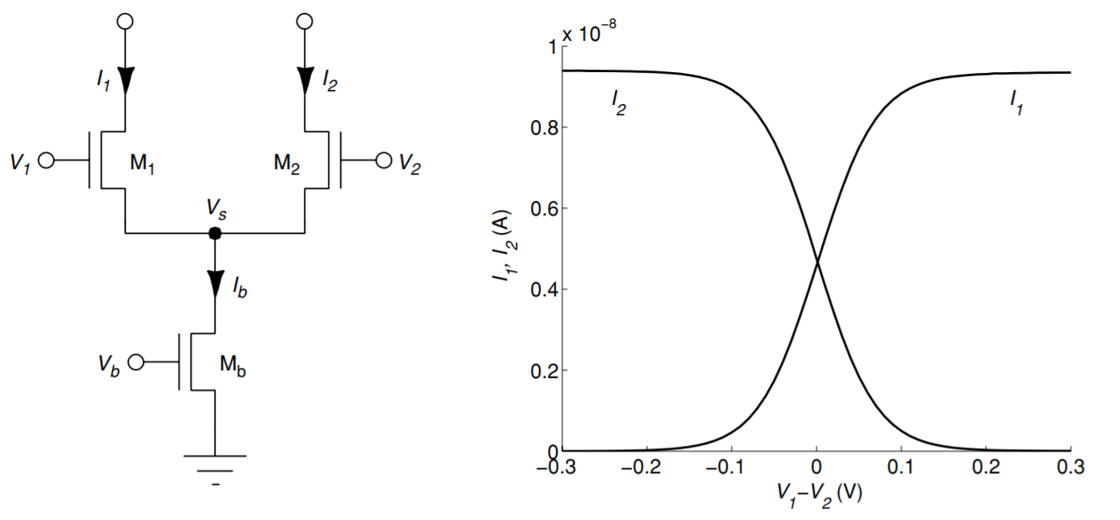
\includegraphics[width=0.85\linewidth]{../../Figures/Differential_Pair.PNG}
    \caption{(A) Differential Pair Circuit. (B) Differential Pair output currents on differential input voltage. Adapted from textbook.}
    \label{fig:Differential_Pair}
\end{figure}

The differential pair has the same basic structure as the source follower, except that the current source, also called the \textit{bias current} $I_b$ is now shared by two MOSFETs $M_1$ and $M_2$ whose sources are connected to the drain of the bias MOSFET $M_b$. The sharing of the current between $M_1$ and $M_2$ depends on their respective gate voltages $V_1$ and $V_2$. If all MOSFETs are operated below threshold and in saturation and we assume that $M_1$ and $M_2$ have the same subthreshold slope factor $\kappa_n$, we obtain the following equations (assuming all transistors work in saturatio):

\begin{equation}
    I_1 = I_0 e^{\frac{\kappa V_1 - V_S}{U_T}}
\end{equation}
\begin{equation}
    I_2 = I_0 e^{\frac{\kappa V_2 - V_S}{U_T}}
\end{equation}

Because of Kirchoff's Current Law, $I_B = I_1 + I_2$, and $I_B = I_1 + I_2 = I_0 e^{\frac{\kappa V_b}{U_T}}$. Now we can rewrite $I_b$

\begin{equation}
    I_b = I_0 e^{\frac{-V_S}{U_T}} (e^{\frac{\kappa V_1}{U_T}} + e^{\frac{\kappa V_2}{U_T}})
\end{equation}

With some algebra (by factoring out $e^{\frac{-V_S}{U_T}}$), we can reach the elegant rewriting of $I_1$ and $I_2$ as a function of the two input voltages:

\begin{equation}
    I_1 = I_b\frac{e^{\kappa_n V_1/U_T}}{e^{\kappa_n V_1/U_T + e^{\kappa_n V_2/U_T}}}
\end{equation}
\begin{equation}
    I_2 = I_b\frac{e^{\kappa_n V_2/U_T}}{e^{\kappa_n V_1/U_T + e^{\kappa_n V_2/U_T}}}
\end{equation}

Now if we take the difference between $I_1$ and $I_2$: 

\begin{equation}
    I_1 - I_2 = I_b\frac{e^{\frac{\kappa V_1}{U_T}} - e^{\frac{\kappa V_2}{U_T}}}{e^{\frac{\kappa V_1}{U_T}} + e^{\frac{\kappa V_2}{U_T}}} = I_b \mathrm{tanh}(\frac{\kappa (V_1 - V_2)}{2U_T}) 
\end{equation}

The dependence of these two currents on the difference of the two input voltages is shown in Figure \ref{Differential_Pair}.B. The curves have a sigmoidal shape \footnote{Sigmoid are very important functions in Neural Networks. You can read a bit more about them here: https://machinelearningmastery.com/a-gentle-introduction-to-sigmoid-function/}. Actually, if you re-arrange any of these two equations, you obtain exactly the form of a sigmoid function \footnote{$I_1 = I_b\frac{e^{\kappa_n V_1/U_T}}{e^{\kappa_n V_1/U_T + e^{\kappa_n V_2/U_T}}} = I_b\frac{1}{1+ e^{\frac{\kappa (V_2-V_1)}{U_T}}}$, which is a sigmoid function with $x = -\frac{\kappa (V_2-V_1)}{U_T}$}. They are almost linear for small voltage differences and saturate at $I_b$ for large voltage differences. We saw that the difference between $I_1$ and $I_2$ gives a tanh function. Such compressive nonlinearities (the sigmoid and tanh) are very useful for the implementation  of different functions, especially in the context of neural networks. What makes the circuit even more useful is the fact that to a first approximation (neglecting the Early effect), the output currents depend only on the difference of the input voltages: The circuit has a small \textit{common-mode} sensitivity. Here is a summary of things about Differential pairs that you want to keep in mind if you get to talk about it in the exam: 
\begin{itemize}
    \item These equations work assuming all transistors operate in subthreshold and saturation.
    \item The assumption that $M_b$ works in saturation should normally not be taken. We should use the full equation to evaluate the current $I_b$. However, in this chapter we chose to just assume this. We will, in the next chapter on Transconductance amplifier, specifically derive the condition that need to be satisfied for $M_3$ to operate in saturation (that is $V_S > 4U_T$, which will yield a specific $V_1$, $V_2$ and $V_b$ relation to satisfy. Don't worry about this too much for now, it will make sense in the next chapter. 
    \item The dependence of these two currents on the difference of the two input voltage gives nice and smooth sigmoid functions, with a linear I-V relationship for small voltage differences. You can use this property to implement programmable resistors in the circuit!
    \item Given that voltages are differential rather than absolute quantities such a property is very useful, for things such as cancelling out noise.
    \item If you take the difference between $I_1$ and $I_2$, you reach a hyperbolic tangent function. This also gives a linear I-V relationship for small voltage differences, which is a property we will use in the transconductance amplifier. 
\end{itemize}

\newpage
\subsubsection{The current correlator}
\label{section:currentcorrelator}

The current correlator measures the correlation between unidirectional input currents, whereas the bump circuit (which we'll look at just after that) measures the similarity or dissimilarity of input voltages. Both of these circuits have been used in many aVLSI designs. For example, these circuits have been used in a stereoscopic vision system
(Mahowald, 1994) to disambiguate between real and false targets. Both circuits are extensively discussed in Tobi's 1993 paper \cite{delbrueck1993bump}

\begin{figure}[H]
    \centering
    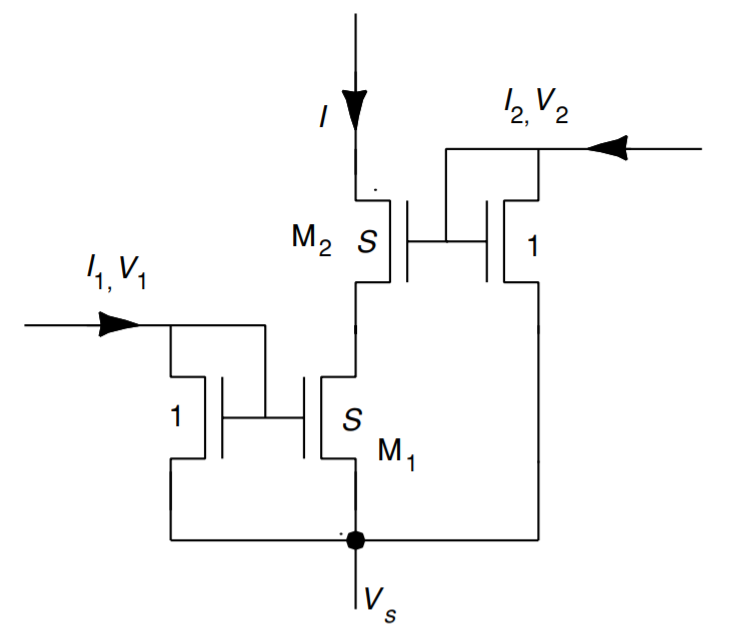
\includegraphics[width=0.5\linewidth]{../../Figures/Current_Correlator.PNG}
    \caption{Current Correlator. Adapted from textbook.}
    \label{fig:current_correlator}
\end{figure}

Carver Mead recognized that in subthreshold operation, the current-correlator circuit
in Figure \ref{fig:current_correlator} computes a measure of the correlation between its two input current $I_1$ and $I_2$. Intuitively, the series-connected transistors perform an analog logic \textbf{AND} like computation. If either of the gate voltages on these series connected transistors is low, then the output current is shut off. Conversely, if both of the input voltages are high, then the output current is large. In the intermediate regions, the circuit computes an approximation to the product of the input currents. Some important details: $M_1$ is in the Ohmic region, and $M_2$ is in saturation. We can thus derive the equations of function for this circuit: As $M_1$ and $M_2$ are connected in series, the same current $I_{out}$ flows through them. 

\begin{equation}
    For \ M_1: I_{out} = I_0e^{\kappa_n V_1/U_T}(e^{-V_S/U_T} - e^{-V/U_T}) = I_0e^{\kappa V_1}(1 - e^{-V}) \ as \ V_S = 0 
\end{equation}
\begin{equation}
    For \ M_2: I_{out} = I_0e^{\kappa_n \frac{V_2 - V}{U_T}} 
\end{equation}
For simplicity, let's ignore $U_T$ in the following equations which cancels out anyways. 
We can factor the last equation as follows: 
\begin{equation}
    e^V = \frac{I_0e^{\kappa_n V_2}}{I_{out}} 
\end{equation}
From simple saturation equation, we can derive $I_1$ and $I_2$:
\begin{equation}
    I_1 = I_0 e^{\kappa V_1}; \$I_2 = I_0 e^{\kappa V_2}
\end{equation}

After some tedious algebra and rearranging, we find back the elegant equation: 

\begin{equation}
    I_{out} = \frac{I_1 I_2}{I_1 + I_2}
\end{equation} 

\subsubsection{The Bump-antibump circuit}
\label{section:bumbantibumb}
The bump anti bump circuit is a circuit pretty much invented by Tobi, that also aims at computing the similarity and difference between two input signals. While we do not need to know the details of the circuit, it is useful (and interesting) to describe qualitatively what computation this rather complex circuit does. 

\begin{figure}[H]
    \centering
    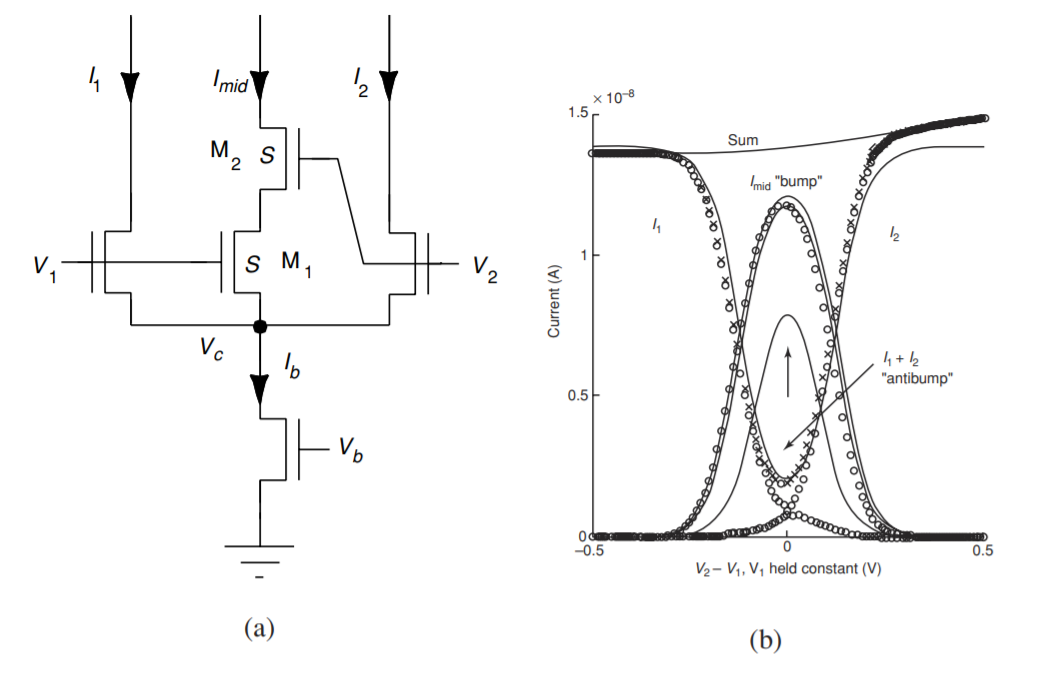
\includegraphics[width=0.85\linewidth]{../../Figures/Bump_Antibump.PNG}
    \caption{(a) Bump-Antibump circuit. (b)  Output characteristics of bump-antibump.  circuit. Adapted from textbook.}
    \label{fig:basalandcerebellum}
\end{figure}

We see hyperbolic cosine functions on the graph (which look like gaussians but are not gaussian) computing the similarity of the inputs. If the two inputs are similar, you have a very high output; and if you have dissimilar inputs the output is low. This is with $I_{mid}$, which makes for the "Bump" of the circuit. Alternatively, you could study $I_1$ and $I_2$ combined which are the complement "Antibump" output of the circuit. So you have a circuit which can compute both the similarity and dissimilarity of two signals! THIS EXPLANATION LACKS CLARITY, NEED TO GET BACK TO IT.